\section{System Description: HabitLab}

Studying behavior change requires in-the-wild intervention and observation~\cite{consolvo2008activity}. Inspired by previous CSCW tools for naturalistic data collection~\cite{reinecke2015labinthewild}, we developed HabitLab as a living laboratory to help us understand online behavior change and as a platform to explore novel behavior change designs (Figure~\ref{fig:homepage}). HabitLab is a Chrome browser extension that aims to help users reduce their time spent online on web pages that the user specifies (e.g., Facebook, Twitter, and Reddit). The system is pitched to end users as a tool that explores various different interventions (referred to as ``nudges'') to help them reduce their time on sites.

\begin{figure}[b]
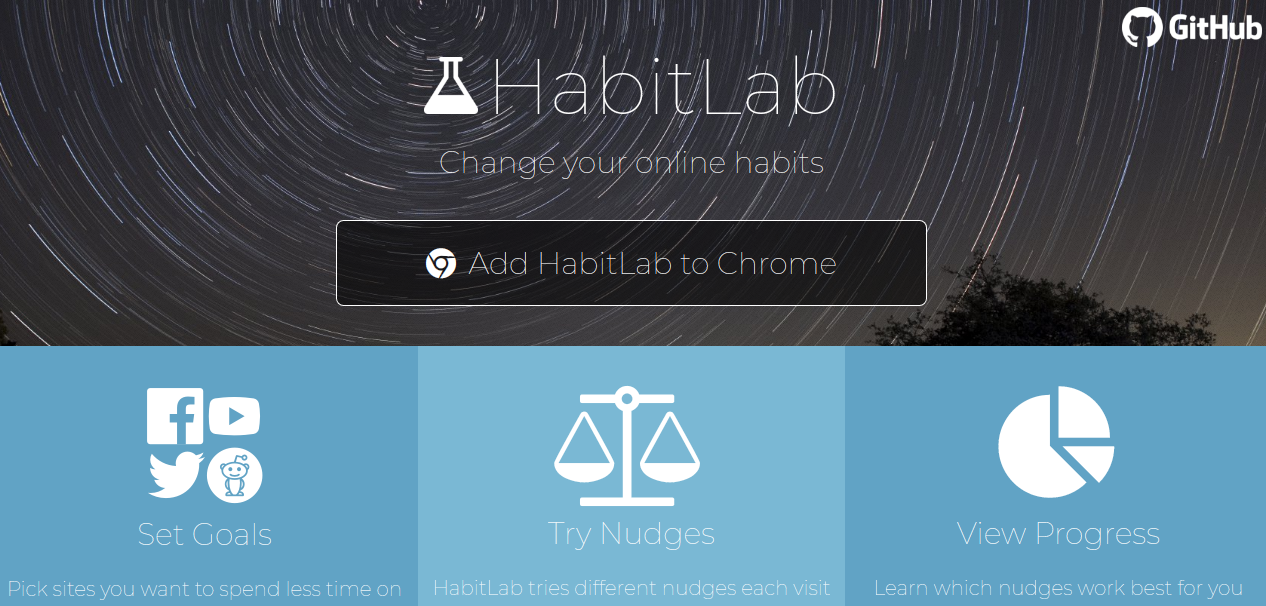
\includegraphics[width=\linewidth]{figures/homepage_cropped}
\caption{HabitLab's homepage describes the browser extension. Users adopt it to try out a large number of different possible interventions, called nudges.}
\label{fig:homepage}
\end{figure}

Users install the extension, and go through an onboarding process where they select sites they wish to reduce their time on (Figure~\ref{fig:onboarding_sites}). There are predefined options---Facebook and YouTube are selected by default, as they were the most commonly used---but users can also add any custom site. Custom sites are suggested via an analysis of the user's browsing history. The system explains to users that they will be shown a variety of interventions (Figure~\ref{fig:onboarding_nudges}), a form of self-experimentation~\cite{Karkar:2017:TFS:3025453.3025480}, to help them reduce time on that site. These interventions are typically targeted to each site, for example a news feed blocker for Facebook or a related video hider for YouTube. However, some interventions such as a stopwatch timer can be added to any custom site. Users can preview the interventions for the sites they select, and enable or disable each intervention if desired. Users can later enable or disable interventions and sites through a settings page.

\begin{figure}
\begin{minipage}[t]{0.49\linewidth}
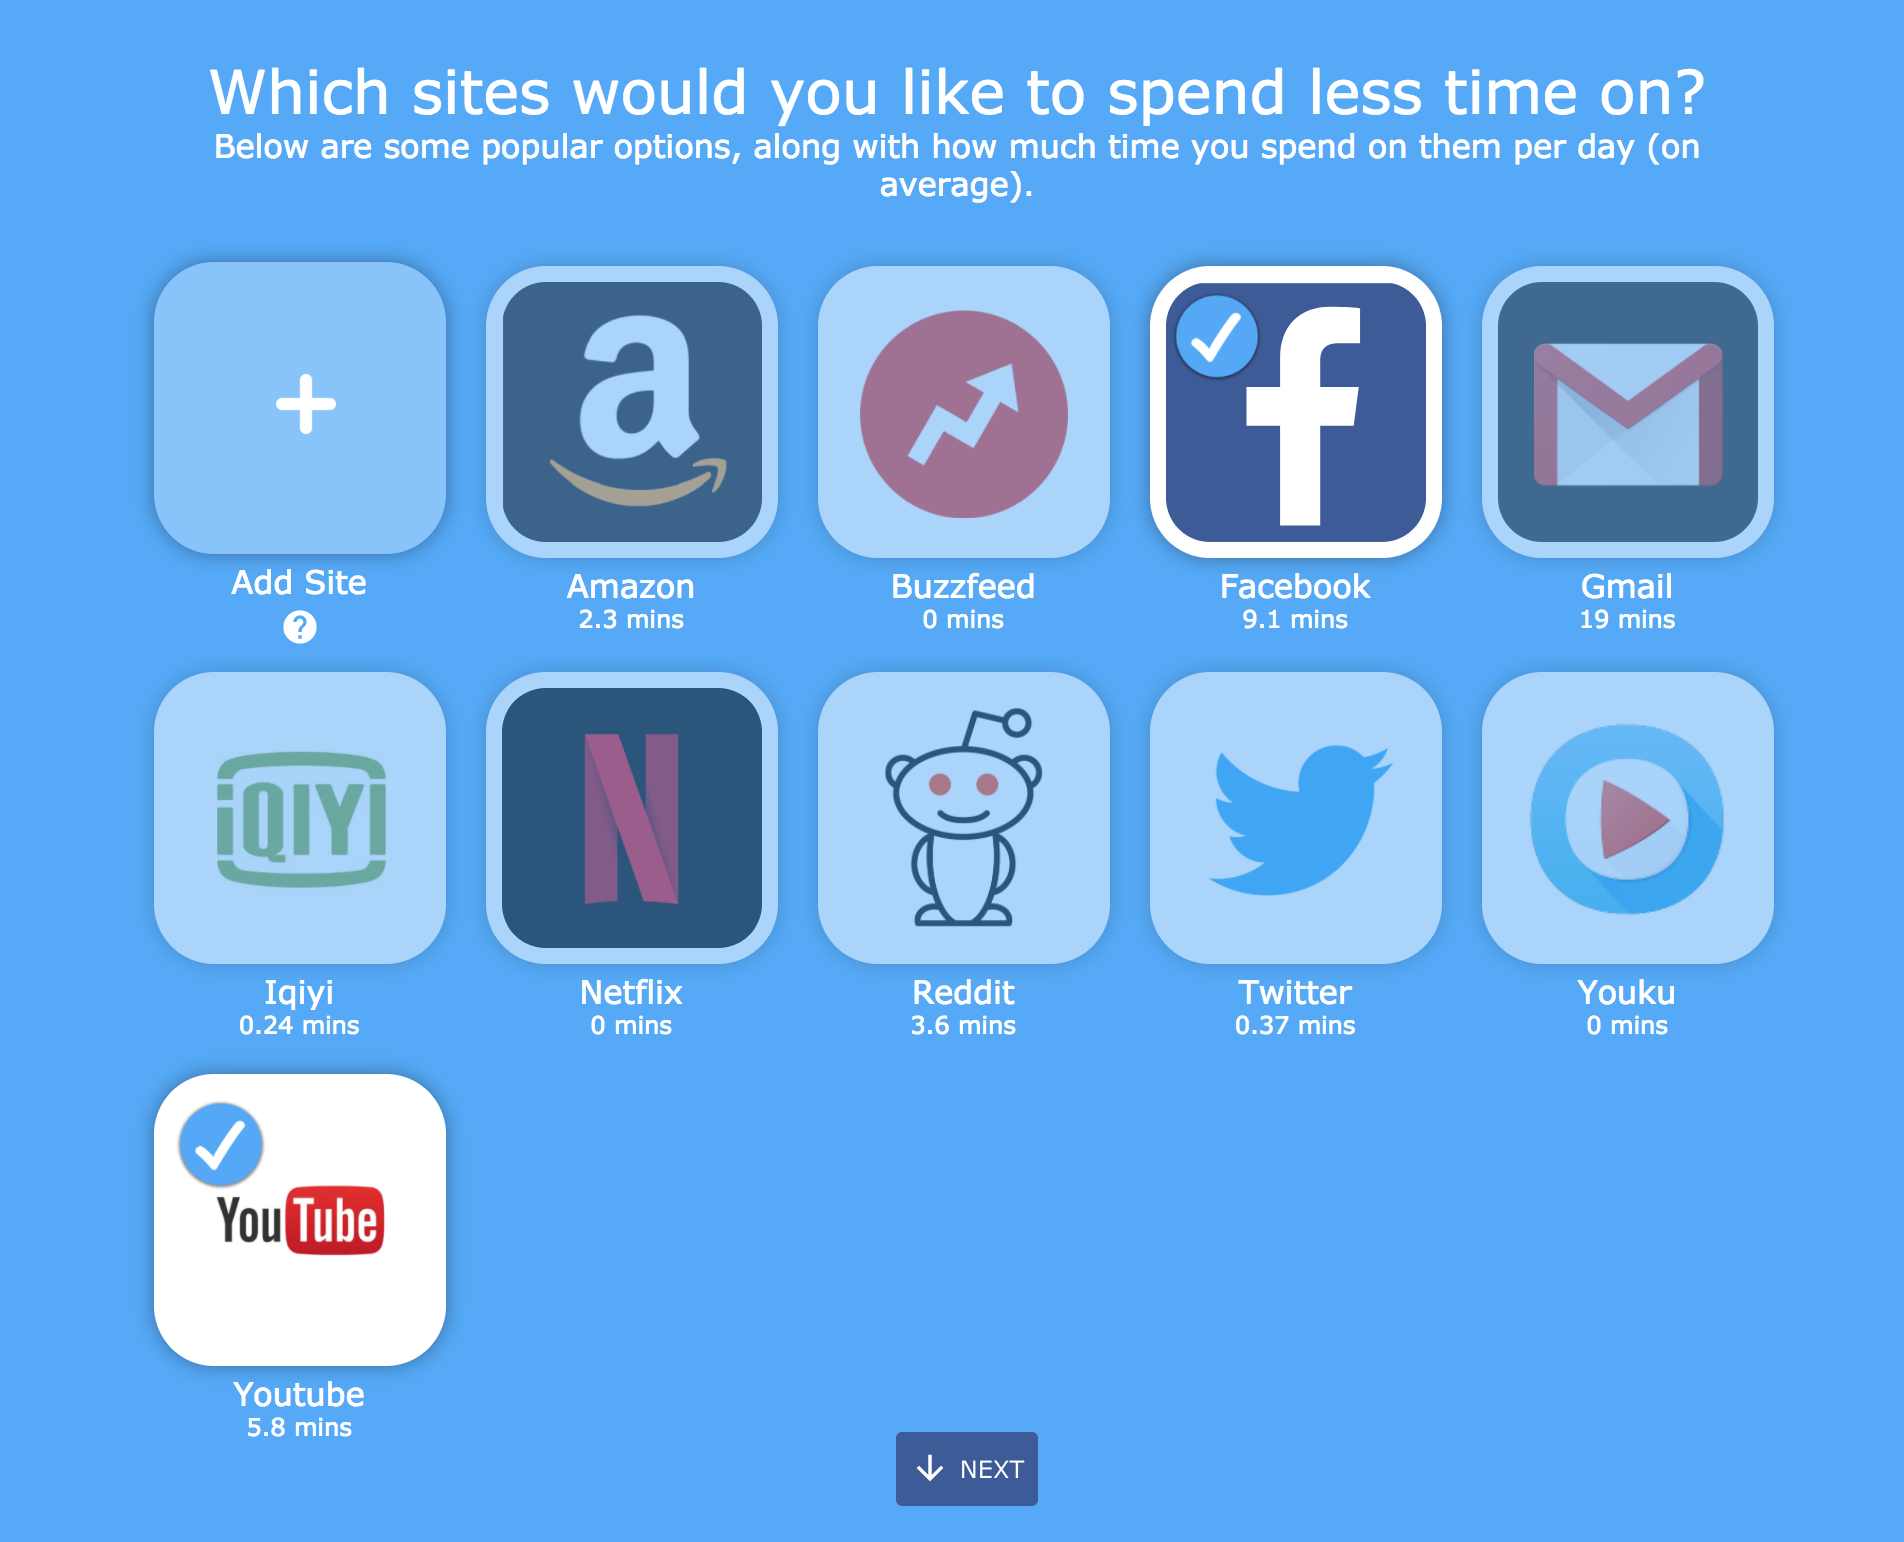
\includegraphics[width=\linewidth]{figures/onboarding_sites}
\caption{During onboarding, users choose which sites they want to spend less time on.}
  \label{fig:onboarding_sites}
\end{minipage}
\hfill
\begin{minipage}[t]{0.49\linewidth}
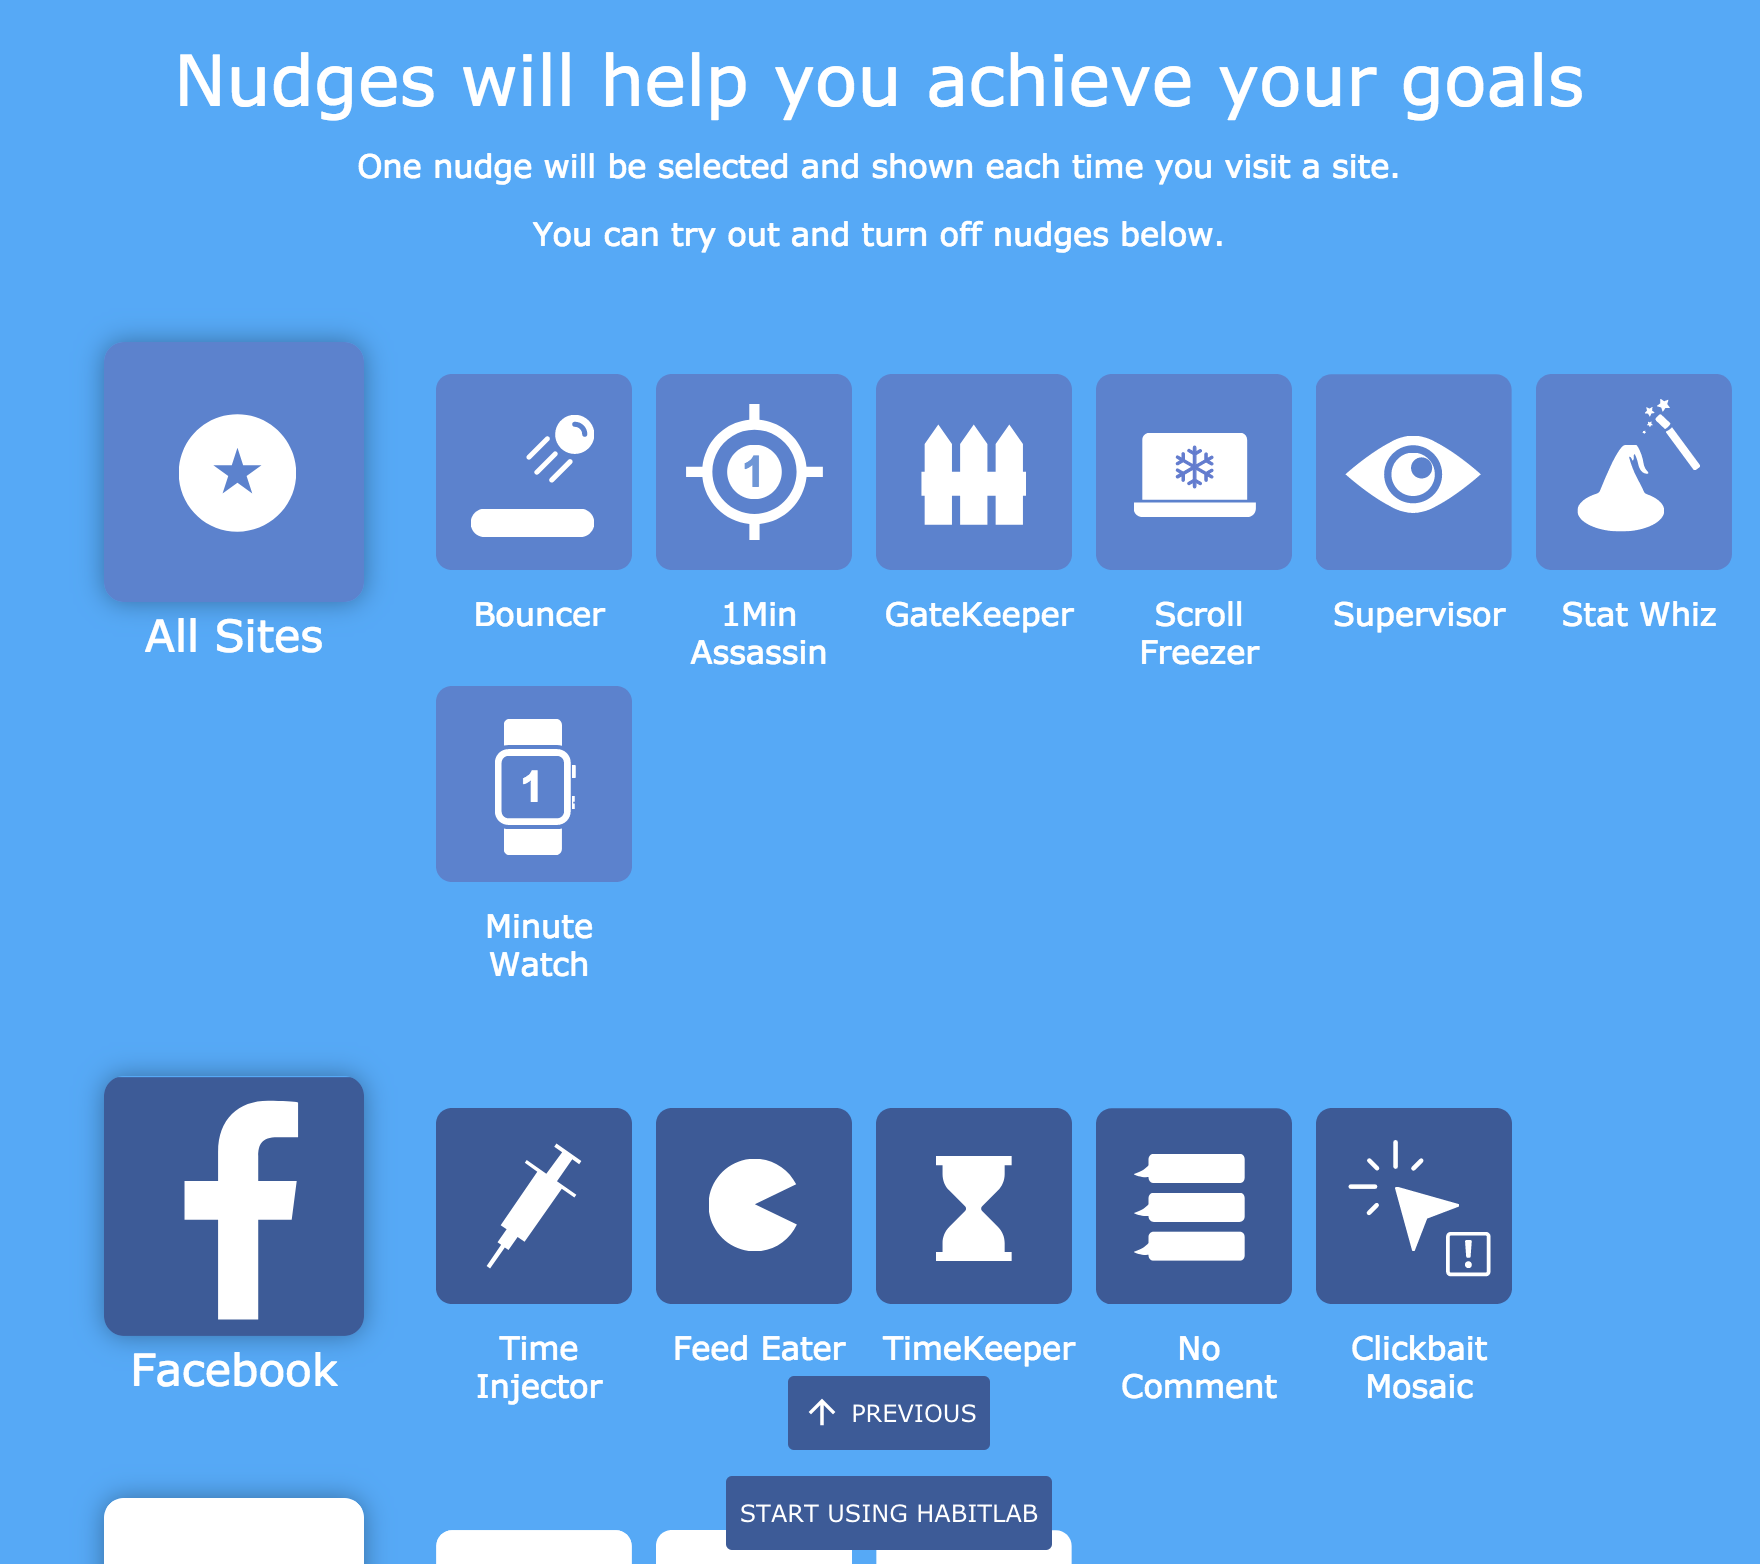
\includegraphics[width=\linewidth]{figures/onboarding_nudges_short}
\caption{Users are presented with the interventions they will see on each site.}
  \label{fig:onboarding_nudges}
\end{minipage}%
\end{figure}

HabitLab emphasizes to users the availability of multiple interventions and that it may show users different interventions each time they load a page. This emphasis is made clear on the HabitLab website, Chrome store listing, and through features in the dashboard such as visualizing the relative effectiveness of different interventions. HabitLab implements a multi-armed bandit algorithm to explore and find the interventions that are most effective for each user, optimizing for minimizing time spent on a site. However, in the experiments in this paper, we disabled this functionality and instead used simple random selection so that we can study the effects of rotation in isolation.

\subsection{Design of HabitLab Interventions}

HabitLab can track time and deploy interventions on all sites, but some interventions are tailored towards specific sites. There are 27 interventions total: seven generic interventions that can be used on all sites, five interventions designed specifically for Facebook, and additional ones designed specifically for YouTube, Reddit, Twitter, Netflix, Gmail, Amazon, iQiyi, and Youku.

Interventions are designed drawing on theories of behavior change---for example, goal setting theory~\cite{locke2002building}, persuasion~\cite{cialdini1987influence,fogg2002persuasive}, and gamification~\cite{deterding2011game}. A sample of the interventions available for Facebook, categorized according to underlying strategies and theories, are shown in Table~\ref{tab:theories}. Screenshots of some Facebook interventions are shown in Figure~\ref{fig:interventions}. %\msb{always use non breaking space \~ between Figure and number, and between sentence and citation block}
% , and health ~\cite{abraham2008taxonomy} \msb{health is not a theory of behavior change}

Not all interventions are enabled by default---this is because some of them have higher attrition rates than others. Non-default interventions can be previewed and enabled by users during onboarding and on the settings page. The interventions enabled by default were the ones we found to have low attrition rates during pilot deployments---we chose this strategy to ensure user retention and growth, which is a prerequisite for gathering data in an in-the-wild experiment setting.

\begin{table}[tb]
\small
\begin{center}
\begin{tabular}{ p{3.3cm} p{3.4cm} p{6.2cm} }
  \textbf{Strategy} & \textbf{Theory} & \textbf{Intervention} \\
  %\hline
  Commitment & Self-consistency theory~\cite{allgeier1979waffle,cialdini1987influence,sherman1980self} & Ask the user to set a goal for the length of time they will stay on the site (generic) \\
  Enforce default limits & Status quo bias ~\cite{samuelson1988status} & Automatically close tab after 60 seconds unless the user clicks a button to ask for more time (generic) \\
%  Enforce default limits & Status quo bias ~\cite{samuelson1988status} & Prevents scrolling unless the user clicks a button to continue scrolling (generic) \\
Reduce social incentives & Social proof~\cite{sherif1935study,cialdini1987influence} & Hide Facebook comments by default (default) \\
  Delaying Rewards & Operant conditioning~\cite{baron1991analyzing} & Make the user wait 10 seconds before visiting Facebook (generic) \\
%  Delaying Rewards & Operant conditioning~\cite{baron1991analyzing} & Shows a page with time spent on Facebook today which they need to click through to get to Facebook (generic) \\
Removing Rewards & Operant conditioning~\cite{baron1991analyzing} & Hide the news feed (default) \\
%  Removing Rewards & Operant conditioning~\cite{baron1991analyzing} & Hide videos and clickbait in the news feed \\
% Gamification & Goal setting theory~\cite{locke2002building}, Flow~\cite{csikszentmihalyi1996flow} & Get points and badges for seeing fewer newsfeed items  \\
  Inform the user & Theory of reasoned action~\cite{ajzen1977attitude} & Show a counter at the top of the page of how long user has been on Facebook today (default, generic) \\
%  Inform the user & Theory of reasoned action~\cite{ajzen1977attitude} & Show a toast notification each minute displaying how long they've been on Facebook today (default, generic) \\
%  Inform the user & Theory of reasoned action~\cite{ajzen1977attitude} & Show a desktop notification each minute displaying how long they've been on Facebook today (generic) \\
% Inform the user & Theory of reasoned action~\cite{ajzen1977attitude} & Inject messages into the news feed showing how long they've been on Facebook today (default) \\
  %Make a plan & Theory of planned behavior \cite{gollwitzer1999implementation} & Ask the user to write out a concrete plan for how they will avoid coming back to the site next time they are tempted to do so \\
  % Rewards/punishment & Operant conditioning~\cite{baron1991analyzing} & Block the site for four hours if the user spends too much time on site in this session \\
  %Stress management & Stress coping~\cite{thoits1995stress} & Reflection on stressors that lead to visiting Facebook \\
  
\end{tabular}
\end{center}
%\vspace{-.7em}
\caption{A subset of the interventions for Facebook, categorized according to persuasion strategy and theory. Interventions that are enabled by default are marked \textit{default}, interventions that are available for all sites are marked \textit{generic}.}
\label{tab:theories}
\end{table}


% todo need to retake these screenshots so they're anonymous
\begin{figure}[tb]
\centering
	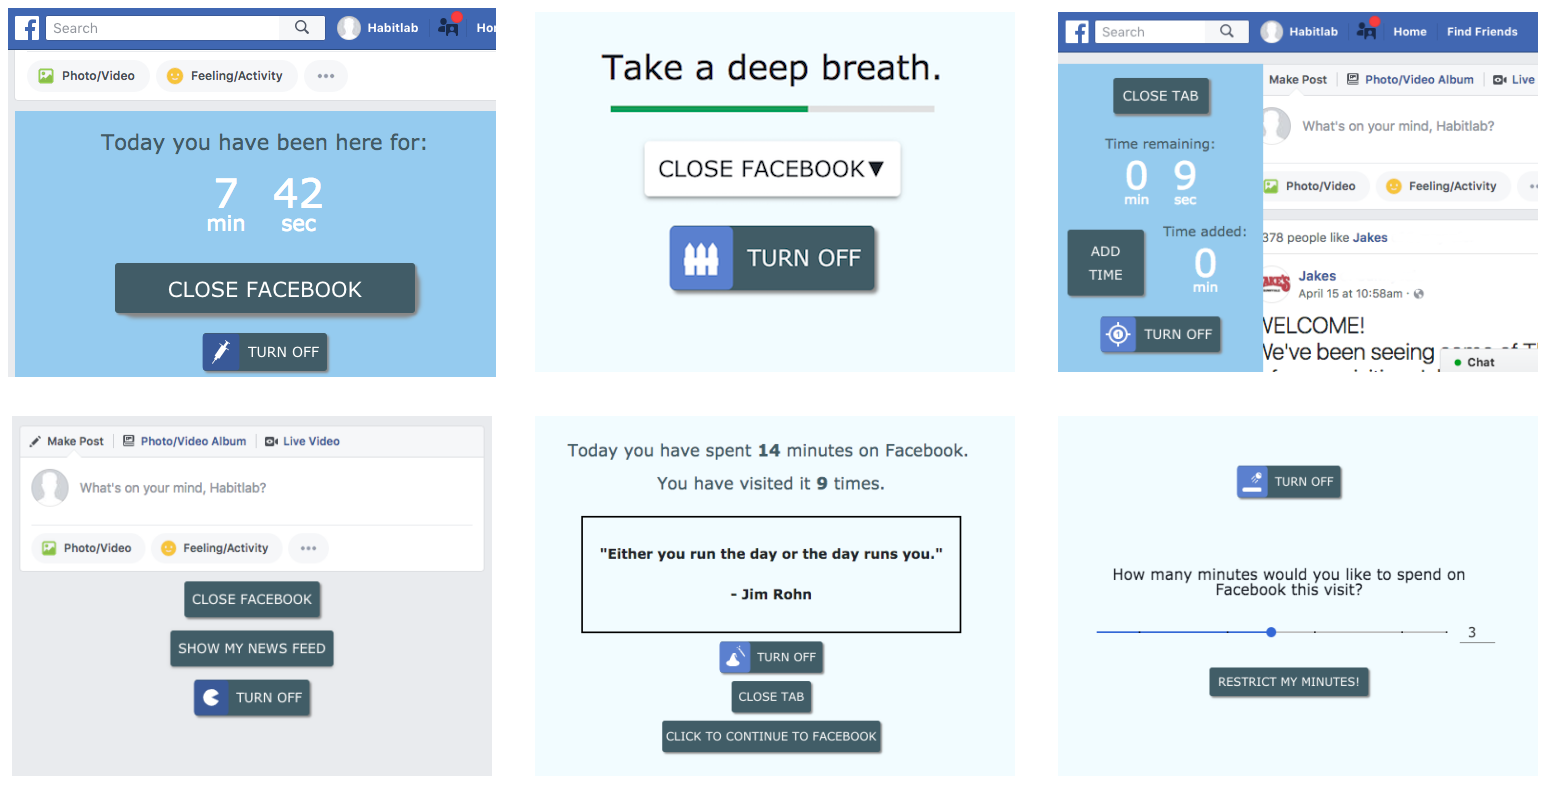
\includegraphics[width=1.0\textwidth]{figures/interventions_new.png}
	\caption{Examples of interventions available for reducing time on Facebook. From left to right, top to bottom: a timer injected into the news feed; a page before opening Facebook requiring that the user wait a few seconds before visiting; a countdown timer that automatically closes the tab after time elapses; an opt-in required to show the news feed; an interstitial page before opening Facebook with a quote; an interstitial page before opening Facebook that requires the user set a time limit for how long they will spend this session.}
\label{fig:interventions}
\end{figure}

\subsection{HabitLab adoption and usage}

As of writing, HabitLab has over \msb{8,000} daily active users from 85 countries (US, India, Germany, France, and the UK are the top 5), and volunteers have translated it into 9 languages (German, French, Spanish, Dutch, Portuguese, Chinese, Czech, Greek, and Turkish).

Users discover the extension through news articles (it has been mentioned in Wired and the New York Times), the Chrome store, or links from an unrelated open-source project by the author. Users are asked to read and provide consent to the research protocol upon installation. They may opt out of data collection if they do not wish to have their data analyzed for research purposes.

% shown in Figure \ref{fig:onboarding_nudges}, some ``generic'' interventions can be used on all sites, and others were developed specifically for a particular site such as Facebook or Youtube.

%\begin{figure}
%  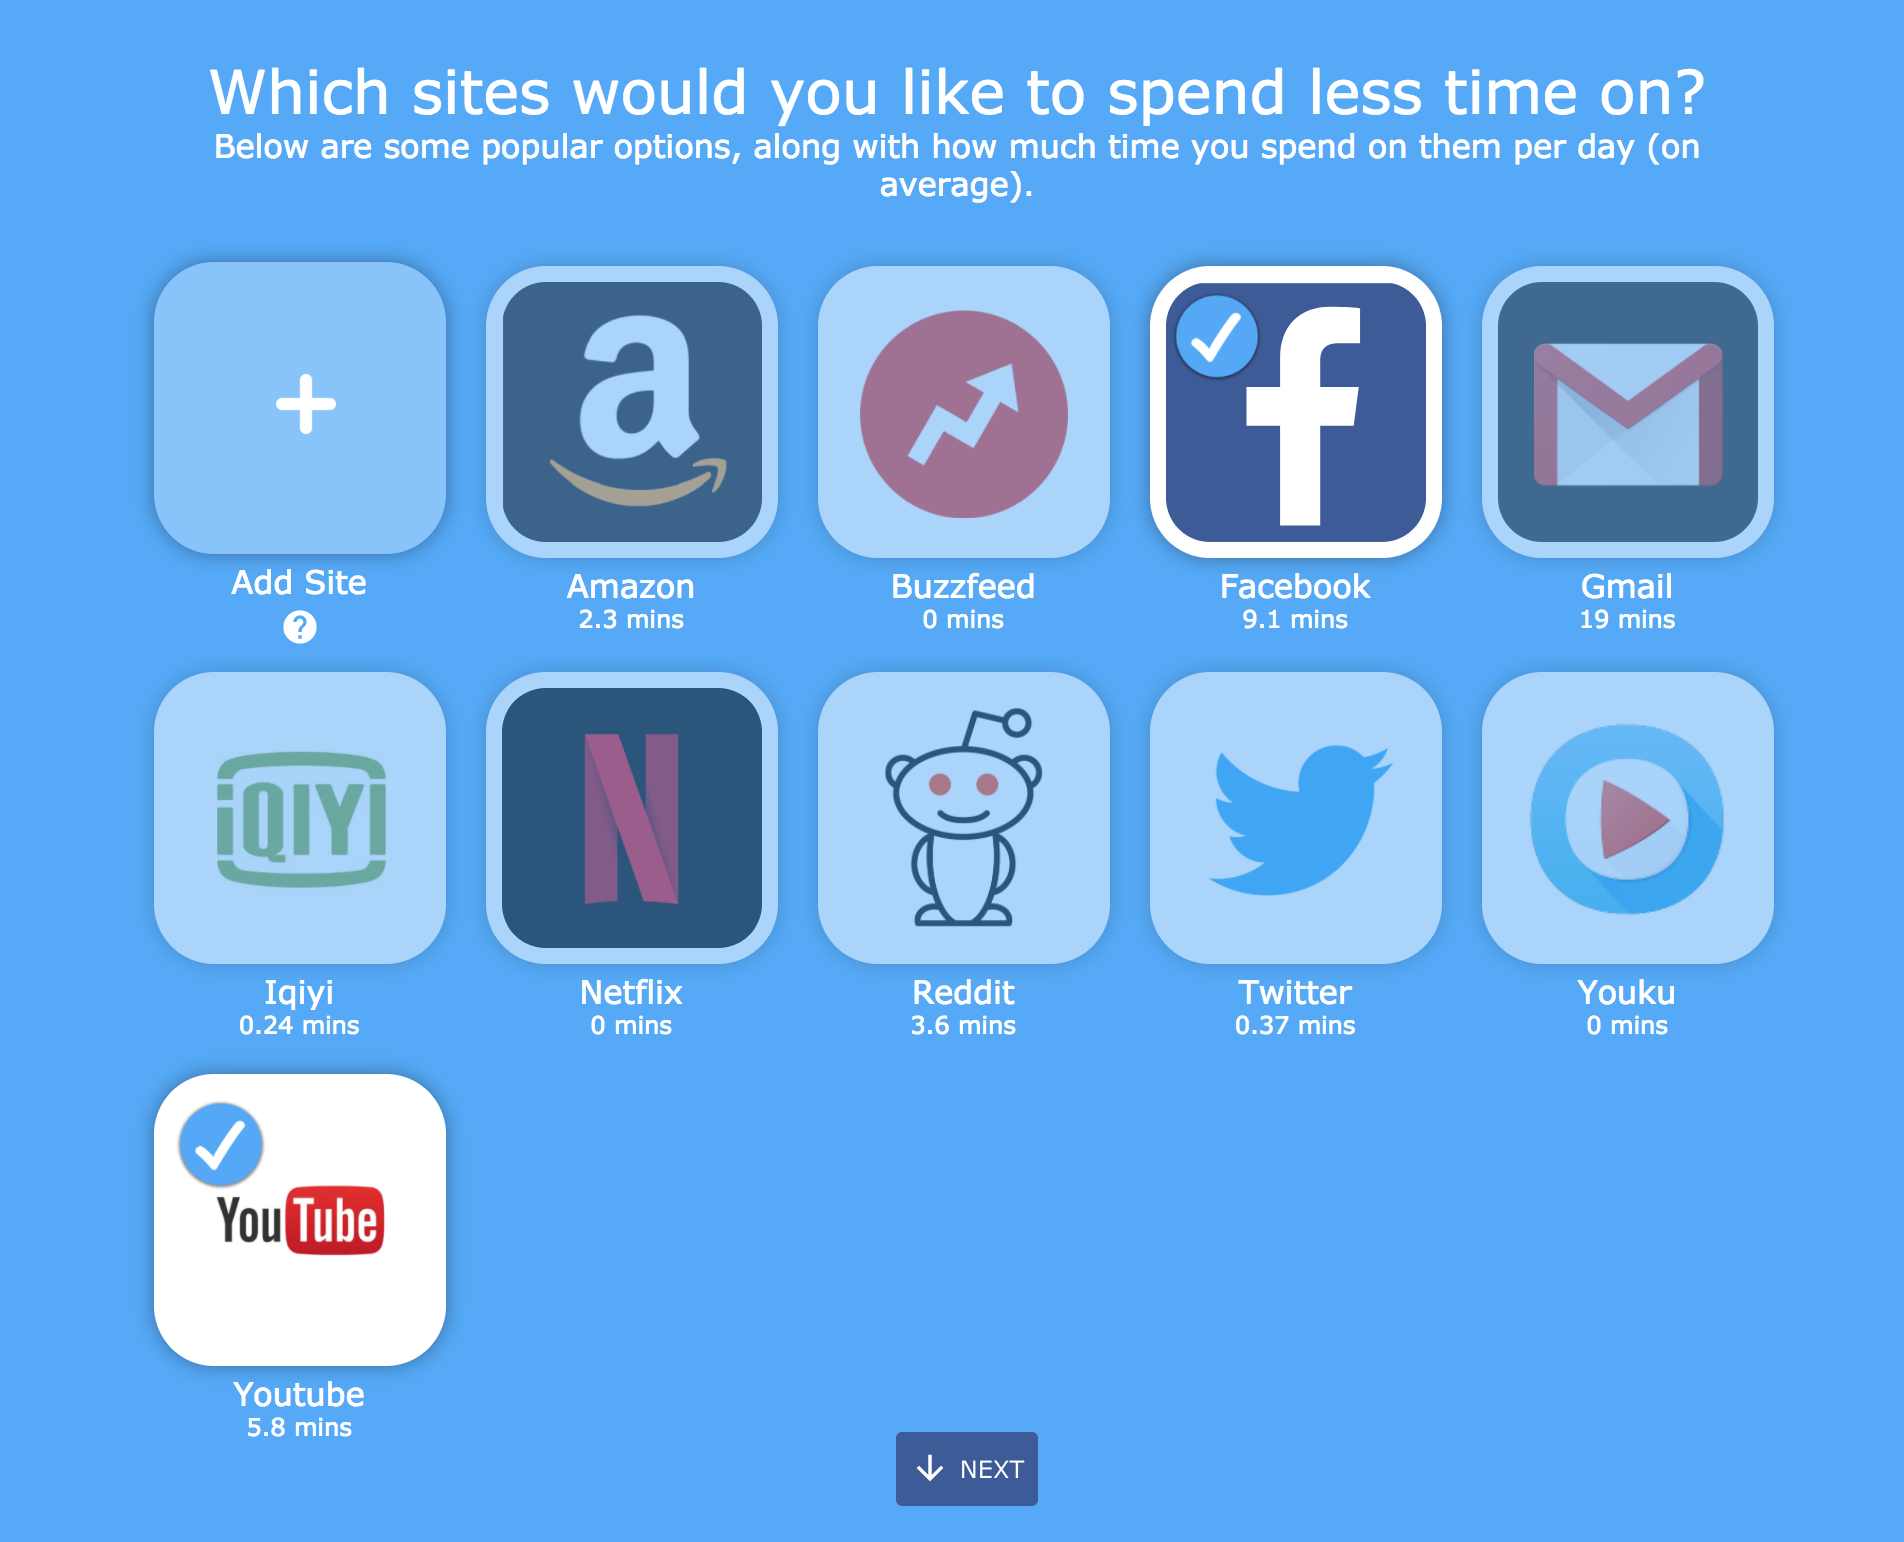
\includegraphics[width=\textwidth]{figures/onboarding_sites}
%  \caption{During onboarding, users first select sites to spend less time on.}
%  \label{fig:onboarding_sites}
%\end{figure}

%\begin{figure}
%  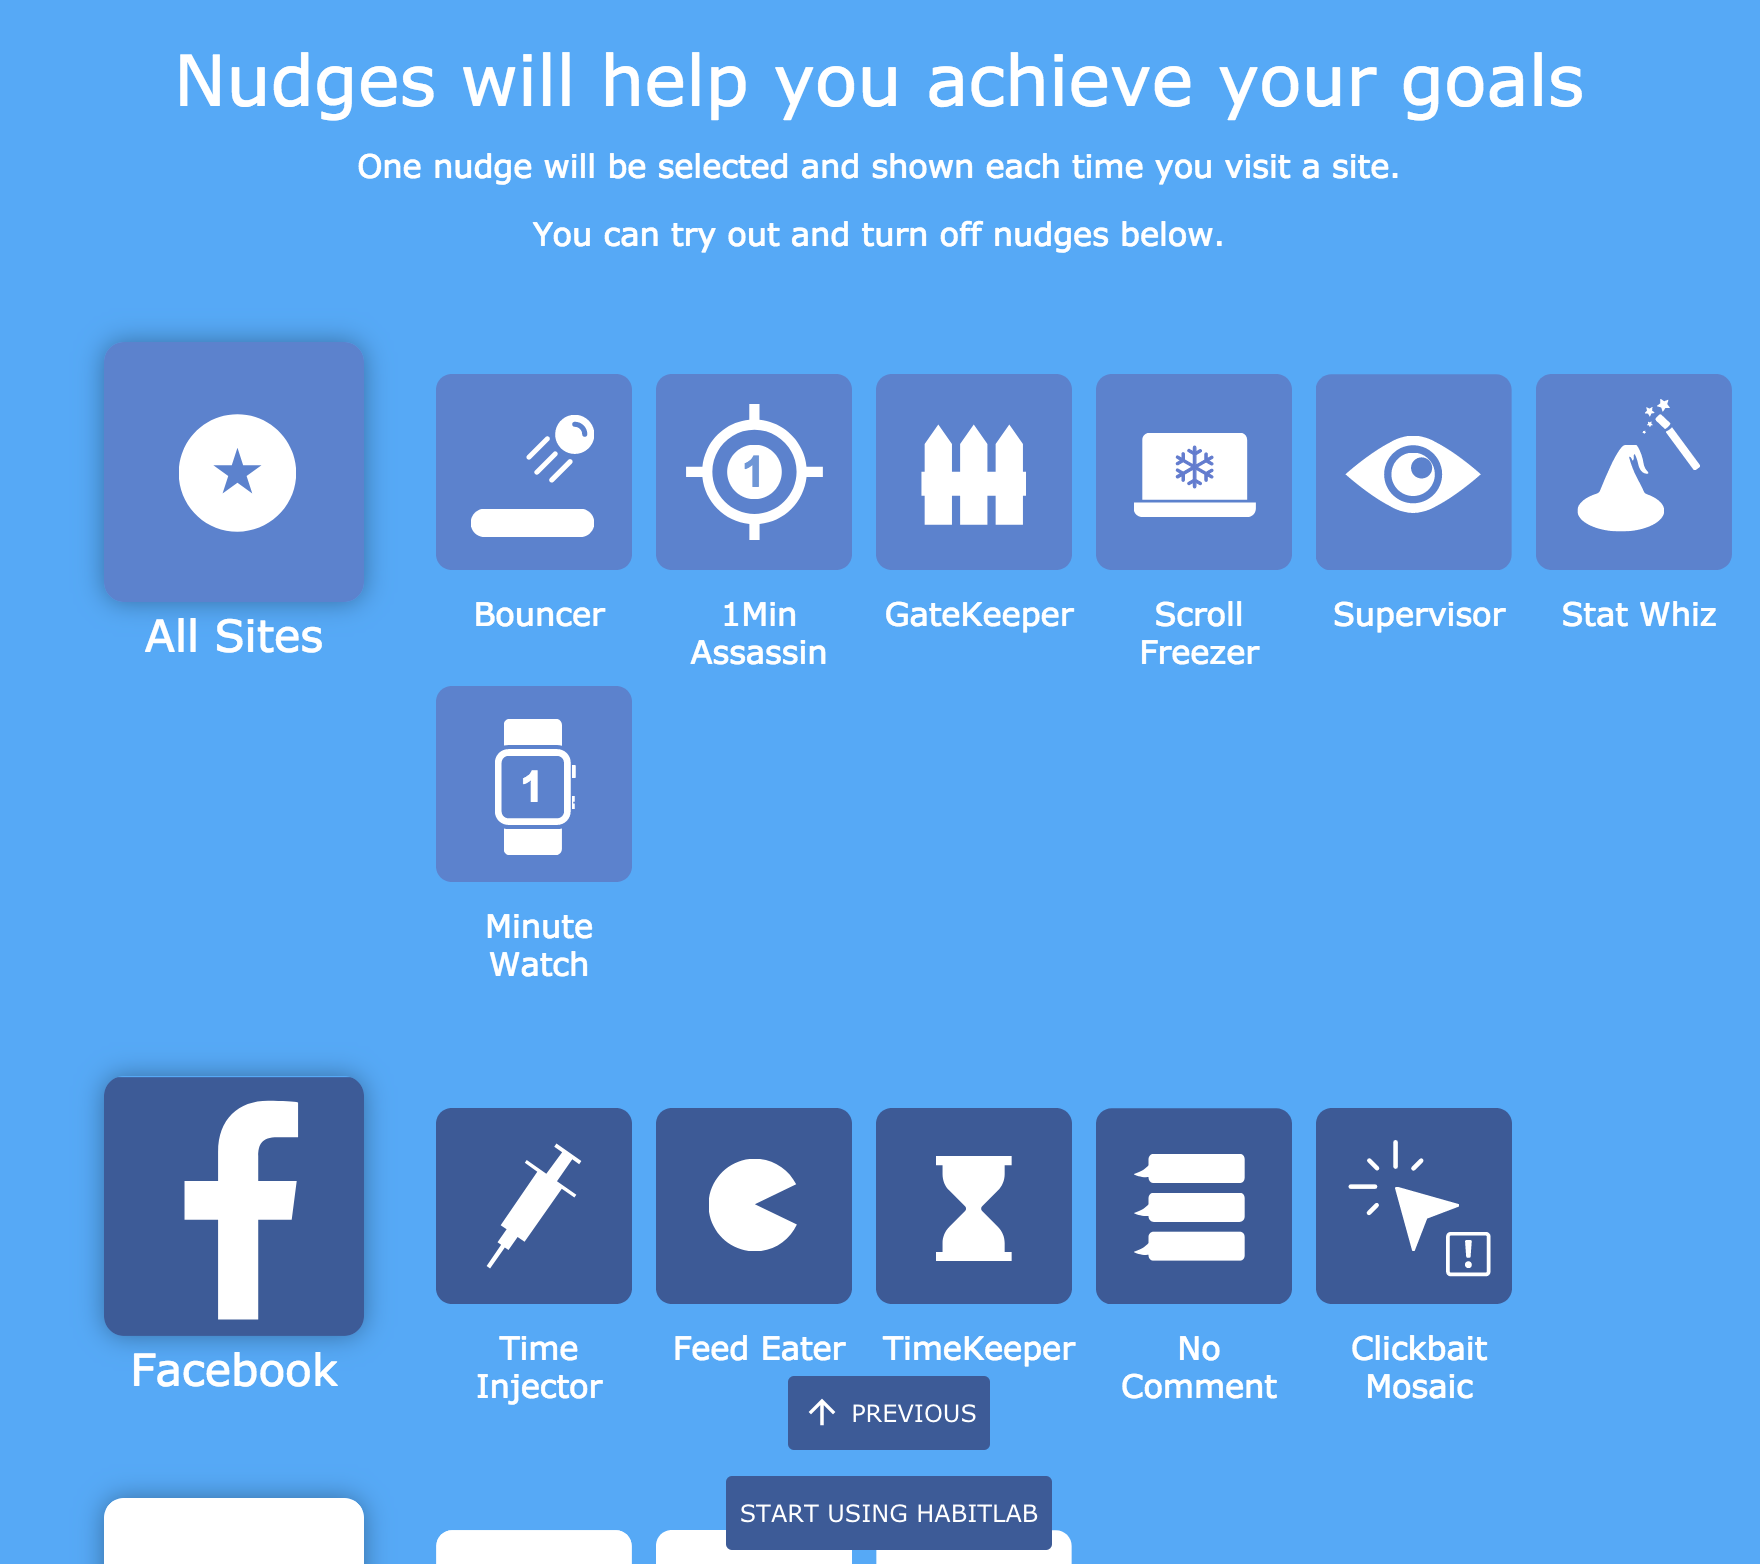
\includegraphics[width=\textwidth]{figures/onboarding_nudges_short}
%  \caption{Users are then presented with the nudges (interventions) they will see on each site.}
%  \label{fig:onboarding_nudges}
%\end{figure}
